% Rules for the HuroCup Lift and Carry Competition
% Jacky Baltes <jacky@cs.umanitoba.ca> 

\documentclass[12pt]{hurocup}

%%
%% iroc_defs.tex
%% Login : <jacky@kaori.wp.shawcable.net>
%% Started on  Wed Apr  7 23:16:07 2010 Jacky (Hansjorg) Baltes
%% $Id$
%% 
%% Copyright (C) 2010 Jacky (Hansjorg) Baltes
%% This program is free software; you can redistribute it and/or modify
%% it under the terms of the GNU General Public License as published by
%% the Free Software Foundation; either version 2 of the License, or
%% (at your option) any later version.
%% 
%% This program is distributed in the hope that it will be useful,
%% but WITHOUT ANY WARRANTY; without even the implied warranty of
%% MERCHANTABILITY or FITNESS FOR A PARTICULAR PURPOSE.  See the
%% GNU General Public License for more details.
%% 
%% You should have received a copy of the GNU General Public License
%% along with this program; if not, write to the Free Software
%% Foundation, Inc., 59 Temple Place, Suite 330, Boston, MA 02111-1307 USA
%%

\newcommand{\thisyear}{2010}

\newcommand{\IROC}{\textsc{IROC}}



\begin{document}

\title{\IROC: Junkyard Challenge\\
  Laws of the Game \thisyear}

\author{Jacky Baltes\\
Autonomous Agents Laboratory\\
University of Manitoba\\
Winnipeg, Manitoba\\
Canada, R3T 2N2\\
Email: jacky@cs.umanitoba.ca\\
WWW: http://www.cs.umanitoba.ca/\~{ }jacky
}

\maketitle

\begin{center}
% \includegraphics[width=0.4\linewidth,angle=-90]{Figures/junkyard_challenge_life2}
 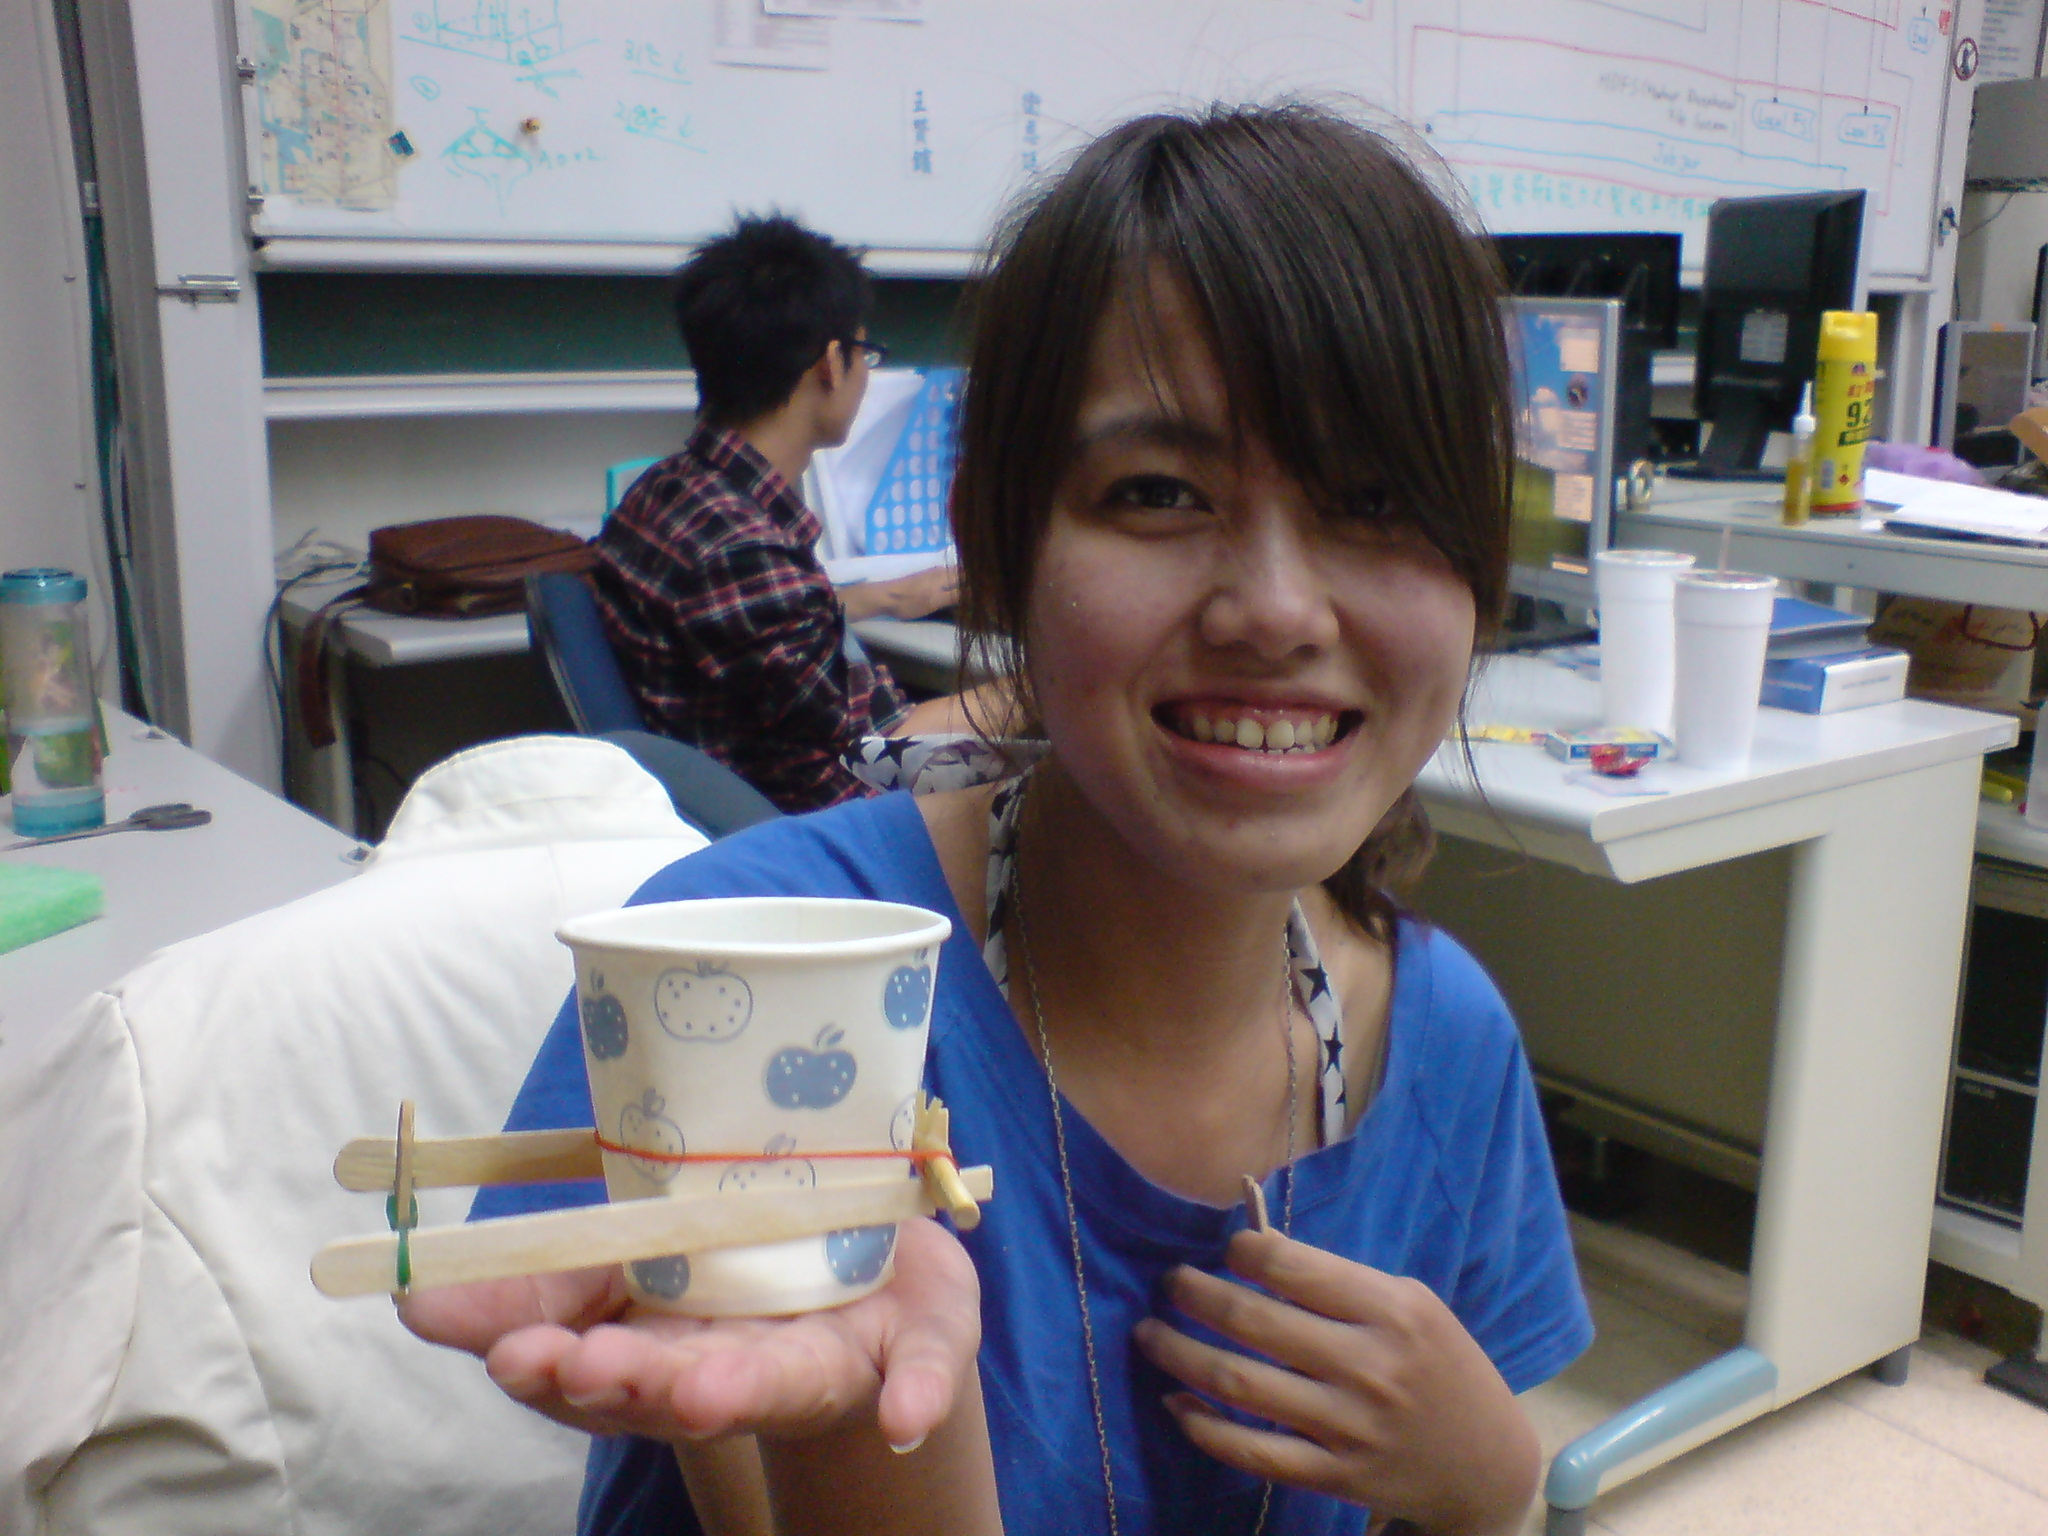
\includegraphics[width=0.7\linewidth]{Figures/junkyard_challenge_life}
\end{center}

\begin{abstract}
The following rules and regulations govern the Junkyard Challenge
competition at the International Robot Olympiad (\IROC) event. The
\IROC\ competition is an International event aimed at increasing
interest in sciences for junior and senior high school students by
exposing them to robotics.
%
The main goal of the junkyard challenge is to provide a competition
emphasizing creativity, imagination, and ¨on the spot¨ problem solving
skills.
%
Teams are given a collection of commonly available components and
tools and are given limited time to design and built a small robot
to solve a particular task.
\end{abstract}

\section*{Latest Version of the Rules for \IROC\ Junkyard Challenge}
\label{sec:updates}

The latest official version of the rules of the game for \IROC\ is
always available from the \IROC\ website (http://www.iroc.net).

This document also includes a set of supplemental regulations which
are the rules and requirements for previously held junkyard
challenges.

Since the participants and their associates must not know the specific
items, tools, and the challenge task before the start of the
construction phase, it is important that this information is kept top
secret until that time.

\section{Junkyard Challenge}
\label{sec:junkyard-challenge} 

The goal of this competition is to provide an event that requires
students to use their imagination and creativity to solve various
problems using commonly available items such as popsicles and rubber
bands and simple tools such as scissors and hammers. The students are
not allowed to use any other items or tools. This levels the playing
field, since teams with more expensive hardware do not have an
automatic advantage.

The students do not know the specific items that will be available,
nor the specific task that they are supposed to solve. Students must
rely on their own problem solving skills rather than being guided by
parents or teachers.

The game is inspired by the exploits of MacGyver (a popular American TV
series in the 80s) and the Junkyard Wars reality TV shows.

\section{Laws of the Game: Junkyard Challenge}
\label{sec:laws-junkyard-challenge}

The following laws describe the specifics of the junkyard challenge
event.

\law[JC]{The Construction Zone}
\label{jc-team}

\begin{lawlist}[JC]

\item Each team has access to a construction zone where they can
  design and built their robot. 

\item The minimum construction zone for each team should be at least
  as big as one table.

\end{lawlist}

\law[JC]{The Field of Play}
\label{lc-field}

\begin{lawlist}[JC]

\item The makeup and dimensions of the playing field depend on the
  exact challenge that students are supposed to solve.

\item During the construction phase, each team can request access to
  the playing field to test their robot. The referee will grant access
  to the field for short periods of time in first come first served
  manner. If a challenge task requires significant setup time for
  testing, the referee may choose instead to create a schedule for
  testing.

\end{lawlist}

\law[JC]{Items and Tools}
\label{law-iteams-and-tools}

\begin{lawlist}[JC]

\item \label{l-items} Before entering the construction zone at the
  start of the competition, each team will be given a set of
  items. See \ref{dec-items} for an example set of items. The set of
  items is not known to the teams before the start of the competition.

\item \label{l-tools} Before entering the construction zone at the
  start of the competition, each team will be given a set of
  tools. See \ref{dec-tools} for an example set of tools. The set of
  items is not known to the teams before the start of the competition.

\end{lawlist}

\begin{figure}
\begin{center}
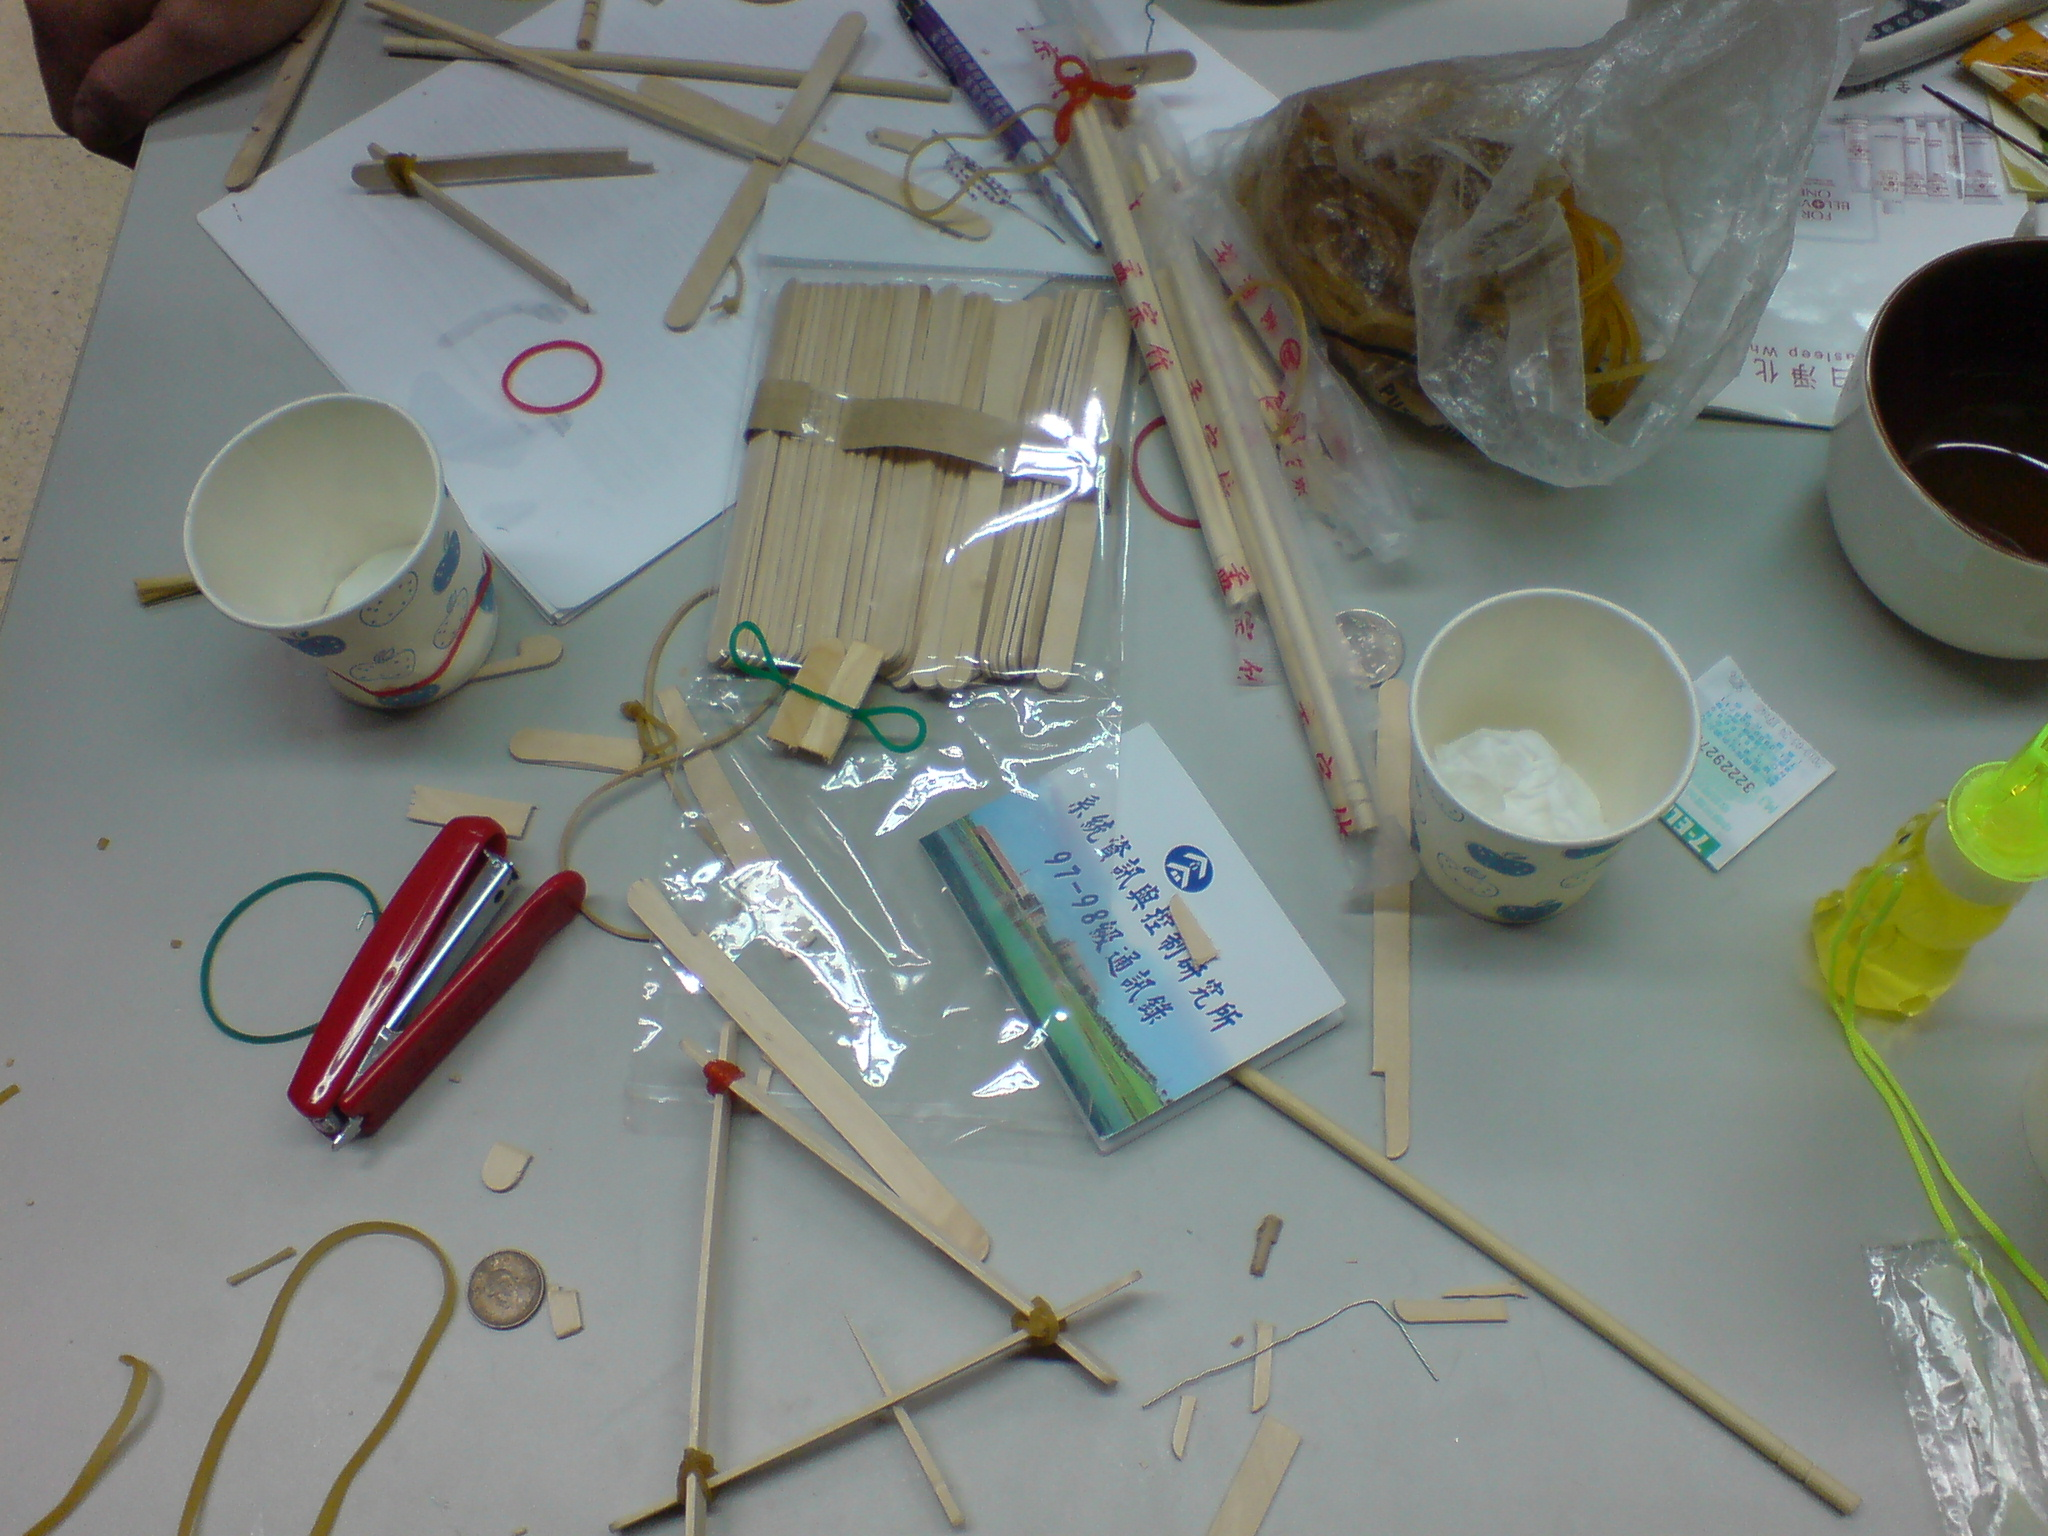
\includegraphics[width=0.8\linewidth]{Figures/junkyard_challenge_table}
\caption{Work Area at the 1st Junkyard Challenge Test Event}
\label{fig:work-area}
\end{center}
\end{figure}

\begin{decisions}

\item \label{dec-items} The organizers try to select commonly
  available items that are safe to be handled by the children. The
  following set of items are examples of commonly available items that
  may or may not be included in the set of items.
  \begin{itemize}
    \item paper, cardboard, laminated paper, styrofoam, 
    \item popsicle sticks, chopsticks, wodden clothes pins,
    \item paper cups, paper plates,
    \item plastic cups, plastic plates,
    \item paper clips, binder clips, hair pins, needles,
    \item wires, strings, ropes, 
    \item scotch tape, duct tape, electric tape,
    \item pens,
    \item cable ties in various sizes,
    \item rubber bands.
  \end{itemize}

  Special purpose items such as ballast tanks, DC motors, gear boxes,
  switches, propellers, resistors, and remote controls may be included
  in the set of items if the organizers deem these materials essential
  to complete the challenge task.
      
  See Fig.\ref{fig:work-area} to see an example of a work area with
  associated items and tools.

\item \label{dec-tools} The organizers try to select commonly
  available tools that are safe to be used by the children. The
  following set of tools are examples of tools that may or may not be
  included in the set of tools

  \begin{itemize}
    \item scissors, 
    \item knives, 
    \item wire cutters,
    \item instant glue, and/or wood glue, 
    \item staplers,
    \item screw drivers,
    \item pliers,
    \item hammers.
  \end{itemize}
  
  Special purpose tools such as soldering irons or drills may be
  included in the set of tools if the organizers deem these materials
  essential to complete the challenge task.

  See Fig.\ref{fig:work-area} to see an example of a work area with
  associated items and tools.

\item This document lists items and tools separately as a convenience
  for organizers. However, the use of tools and items is not limited
  by their classification. For example, a team may choose pliers
  (designated as tools) to add weight to their robot (used as items),
  or use pens (designated as items) to drill holes into popsicle
  sticks (used as tools).

\item The safety of the children is of utmost importance, hence
  dangerous materials (e.g., aggressive chemicals) or tools (band
  saws) may not be handled by the children without supervision of the
  referee or assistants.

\end{decisions}

\law[JC]{Game Play}
\label{law-game-play}

\begin{lawlist}[JC]

\item The junkyard challenge event starts with the construction
  phase. During the construction phase children will enter the
  construction zone and be given a set of items and tools.

\item \label{g-task} After each team has received their set of items
  and tools, the referee will give a brief description of the
  challenge task.

\item \label{g-score} The referee will also give a description of the
  scoring formula being used for this event.

\item \label{g-rule} The referee will also announce any special
  restrictions or rules that may be in effect during the event.

\item \label{g-duration} The referee will also announce the duration
  of the construction phase.

\end{lawlist}

\begin{decisions}

\item An example of possible tasks as described in \ref{g-task} is:
  Build a robot, that
  \begin{itemize}
    \item can carry a 500g weight for 1m,
    \item can dive and pick up the following treasure from the bottom
      of the water pool,
    \item can climb over a 1m tall wall,
    \item and/or can lift a 2kg weight.
  \end{itemize}
\item An example of a scoring rule as described in \ref{g-score} is:
  The robot must carry three metal balls across the water as quickly
  as possible. If a robot looses a ball, then a 60 second penalty will
  be added to the time.

\item The scoring system (see \ref{g-score} must as much as possible
  be based on quantitative performance measures such as time taken to
  complete the task, distance travelled, or weight carried. However,
  in special circumstances, the scoring system may include a knock-out
  competition (e.g., a soccer match) or even a subjective evaluation
  (e.g., judges score the dance performance of a robot).

\item An example of a special rule or restriction as described in
  \ref{g-rule} is: children can have a maximum of five metal pieces
  cut with a band saw by an assistant referee, or the robot must use
  more than three rubber bands.

\item The duration of the construction phase as described in
  \ref{g-duration} is usually \textbf{three hours}. The duration may
  be different for a specific event to obey local constraints and
  requirements.

\end{decisions}

\law[JC]{Infractions and Penalties}

\begin{lawlist}[JC]

\item \label{inf-parents} Only team members are allowed to enter the
  construction zone or the playing field during the competition.

\item \label{inf-team} Team members are not allowed to leave the
  construction zone or the playing field without prior permission of
  the refereee.

\item Any team whose members or associates violate rule
  \ref{inf-parents} to \ref{inf-team} or \ref{g-rule} will be
  disqualified.

\item Any team whose members use additional items except those
  described in \ref{l-items} will be penalized by the referee. The
  sanctions imposed by the referee include time or points penalties
  (for example, the final score is reduced by 30\%), or in serious
  cases may also lead to disqualification of a team. The severity of
  the penalty is decided on the sole discretion of the referee.

\item Any team whose members use additional tools except those
  described in \ref{l-tools} will be penalized by the referee. The
  sanctions imposed by the referee include time or points penalties
  (for example, the final score is reduced by 30\%), or in serious
  cases may also include disqualification of a team. The severity of
  the penalty is decided on the sole discretion of the referee.

\item A team that continues building or modifying their robot after
  the construction phase will be disqualified.

\end{lawlist}

\law[JC]{Method of Scoring}

\begin{lawlist}[JC]

\item At the end of the construction phase, all teams must finish
  building their robot and bring it to the playing field. 

\item At that time, the referee will test the performance of the robot
  and will calculate the resulting score given the scoring formula.

\item 1st, 2nd, 3rd, ... awards will be awarded based on the point
  score. 

\end{lawlist}

\newpage

\section{Supplement 1: Dragon Boat Challenge\\Release Date: 7th June 2010}
\label{sec:supp-dragaon-boat-challenge}

\begin{center}
% 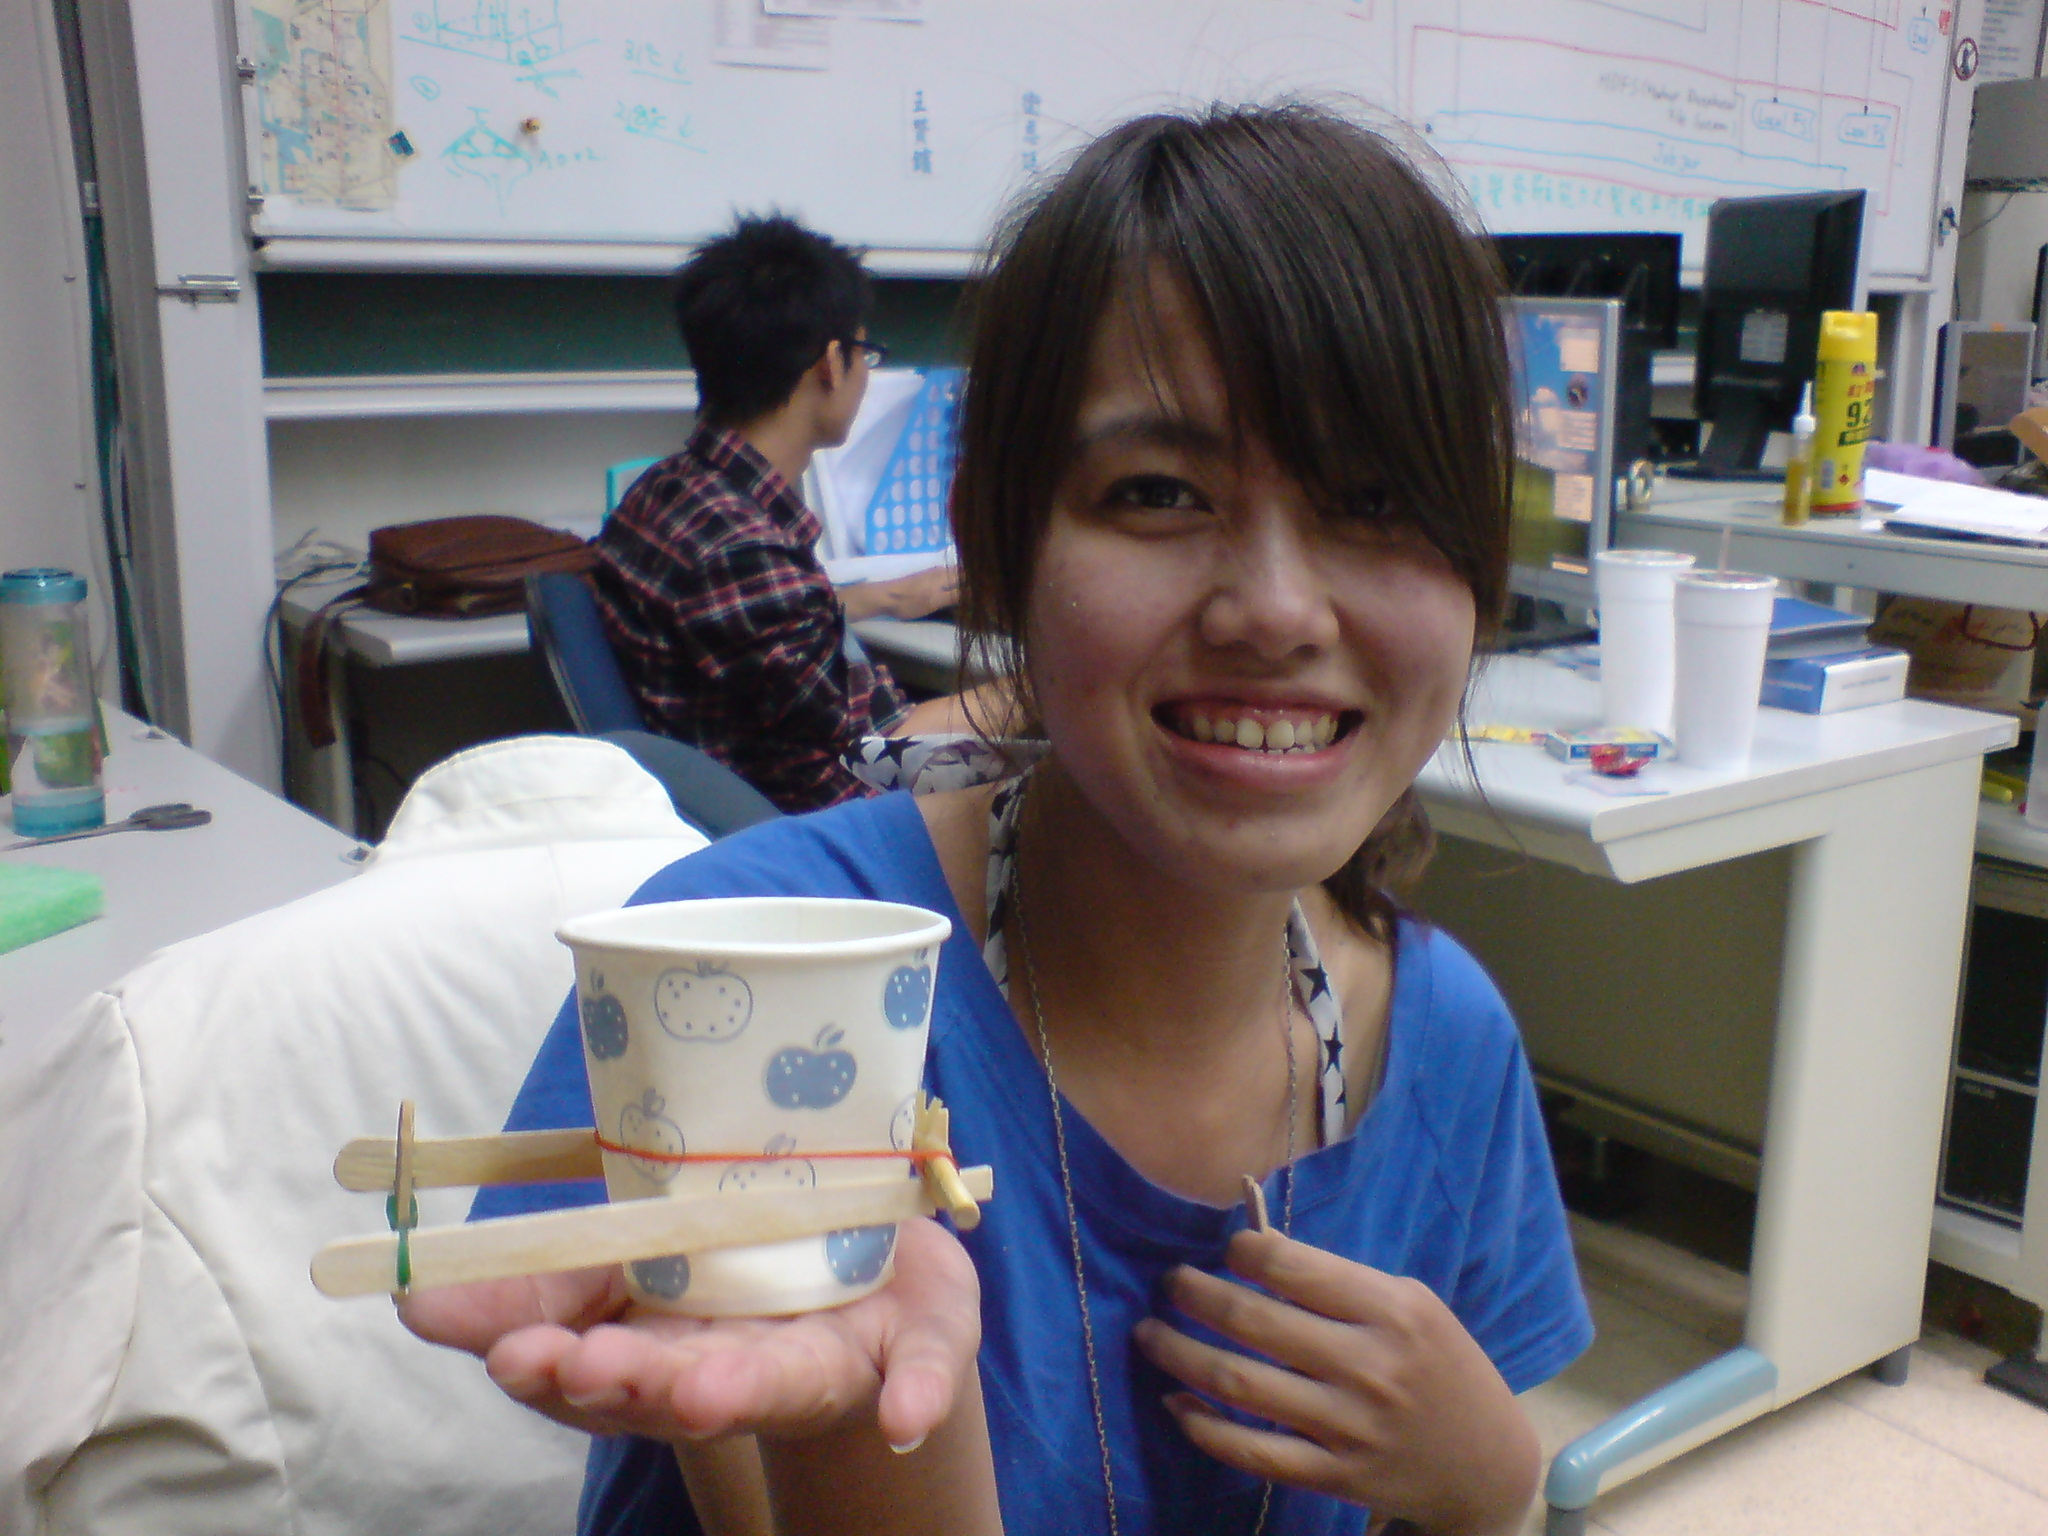
\includegraphics[width=0.7\linewidth]{Figures/junkyard_challenge_life}
\begin{tabular}{cc}
 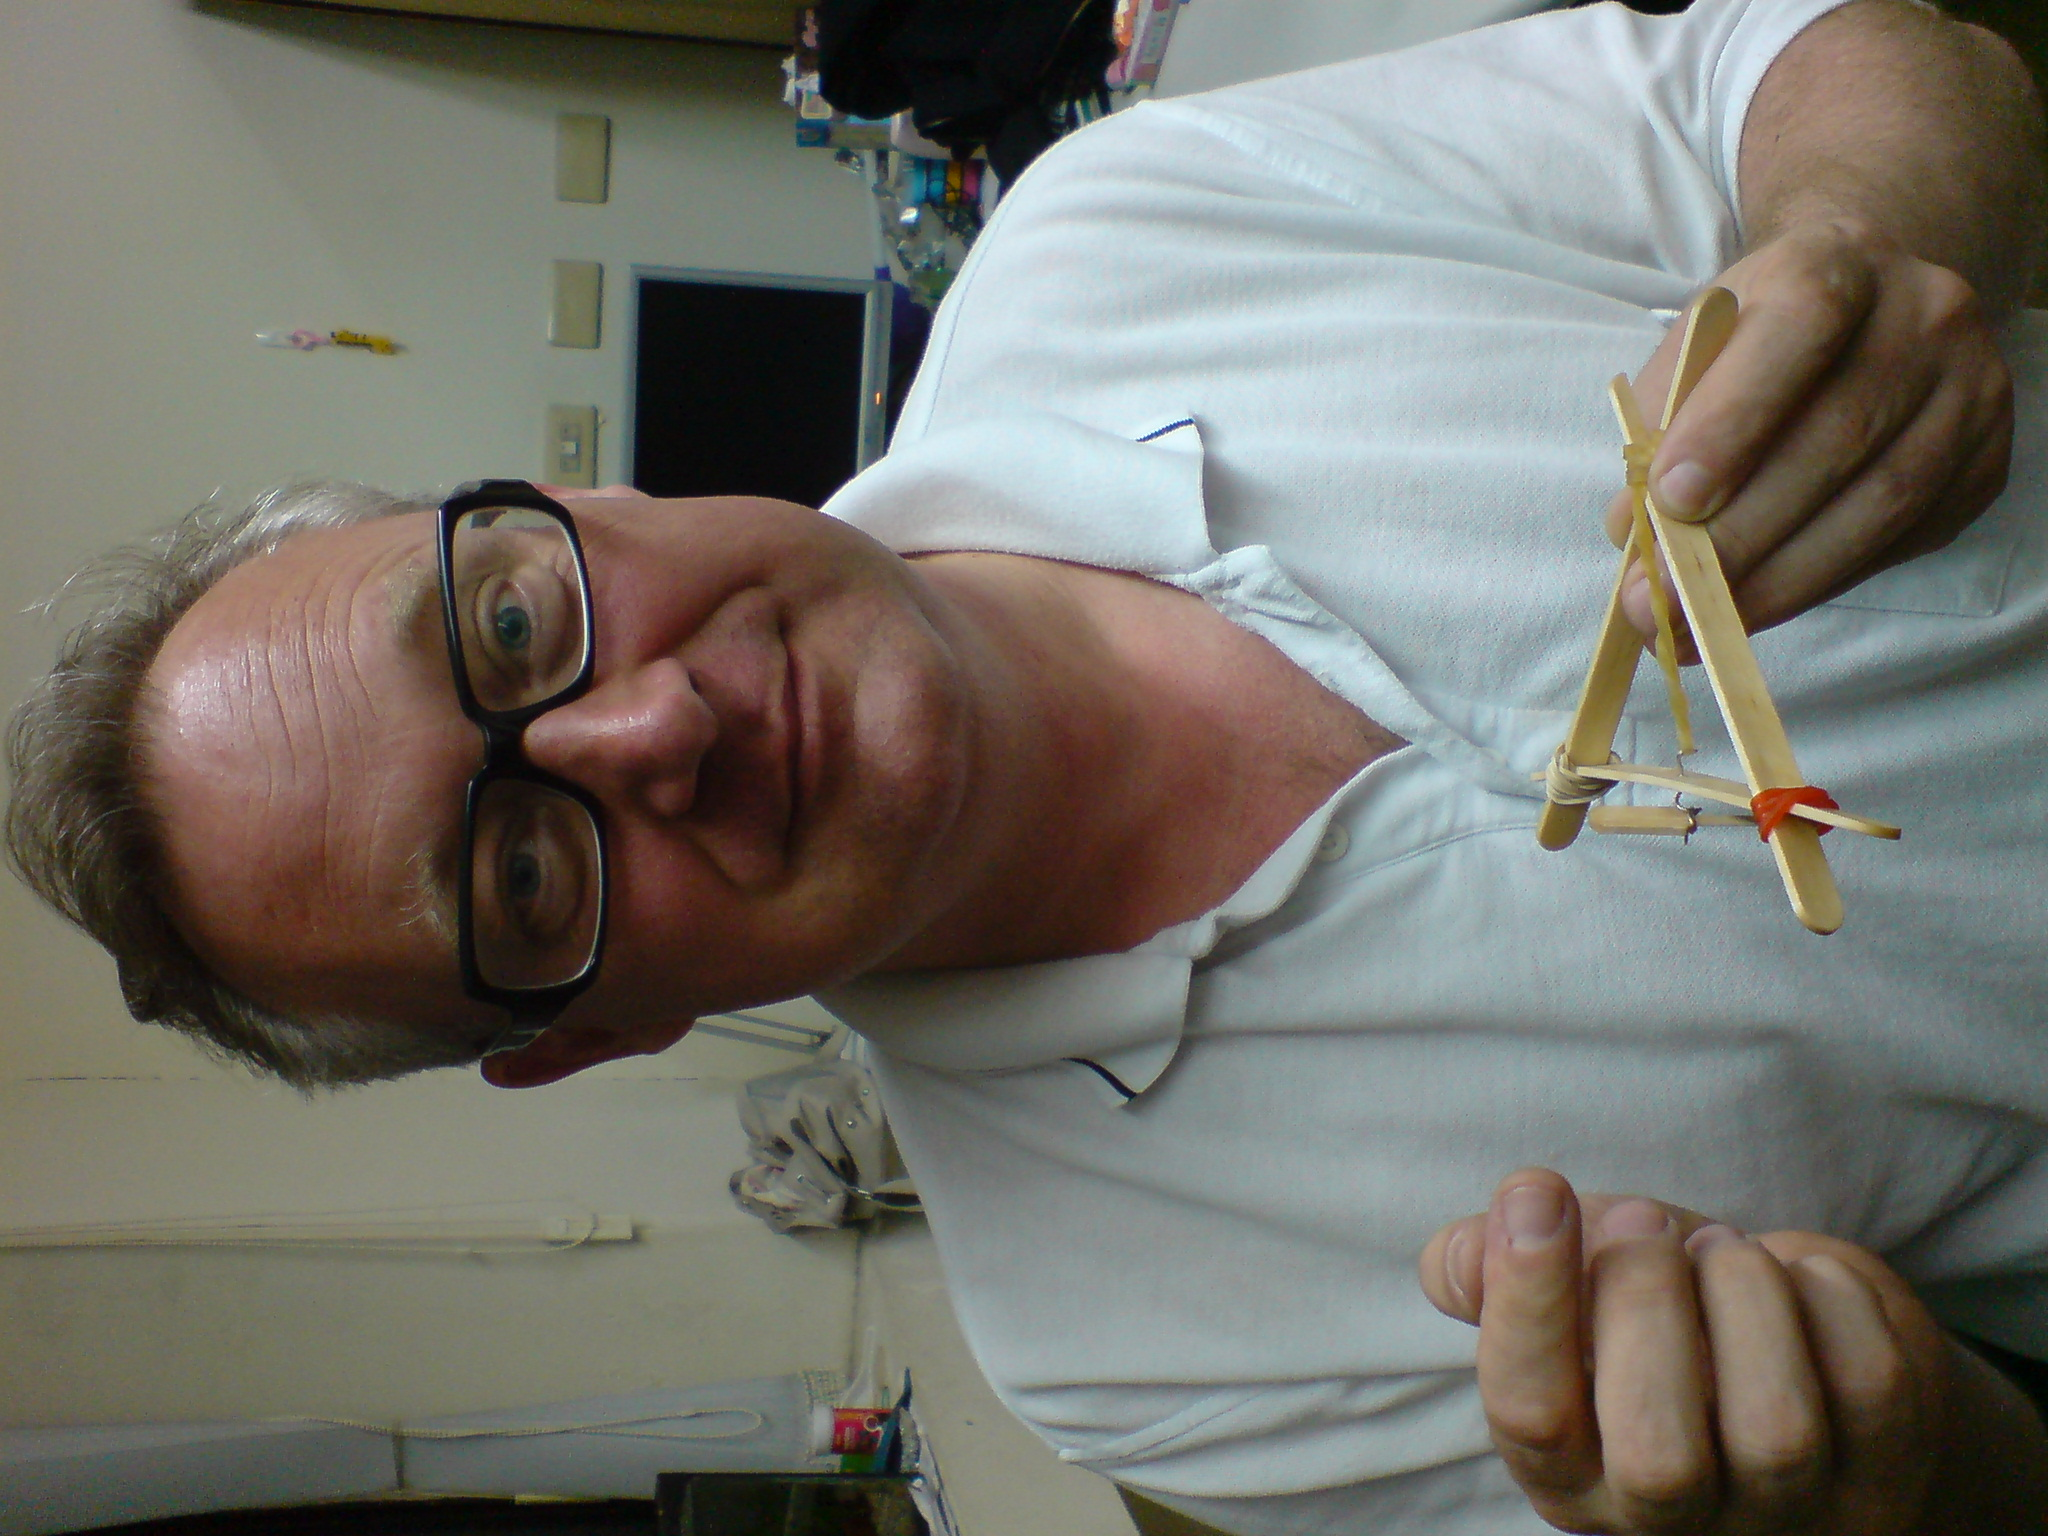
\includegraphics[width=0.4\linewidth,angle=-90]{Figures/junkyard_challenge_life3} &
 \includegraphics[width=0.4\linewidth,angle=-90]{Figures/junkyard_challenge_life2}\\
\end{tabular}
\end{center}

This challenge is intended for the IRO Taiwan event to be held in
Kaohsiung, Taiwan. Do not release until \textbf{June 7th 2010}.

The theme of the IRO Taiwan 2010 event are the dragon boat races, an
annual Chinese festival that is also held in June.

The dragon boat festival celebrates the life and death of Qu Yuan, a
famous poet and scholar during the Warring States (475-221 BC)
period. According to legend, when Qu Yuan, who was exiled by the
emperor because of false accusations of his political rivals, heard of
the fall of Chu, he committed suicide by throwing himself into the
Miluo River. After the people heard that he had drowned they used
boats to race to scene and threw zongzi rice dumplings into the river
to feed the fish in the hope that Qu Yuan's body will not be eaten by
the fish.

\law[DBC]{The Field of Play}
\label{dbc-field}

\begin{lawlist}[DBC]

\item The playing field consists of a kiddie pool with a minimum
  diameter of 2m. See Fig.~\ref{fig:kiddie-pool} for an example.

\begin{figure}
\begin{center}
\begin{tabular}{cc}

\includegraphics[width=0.4\linewidth]{Figures/kiddie-pool} &
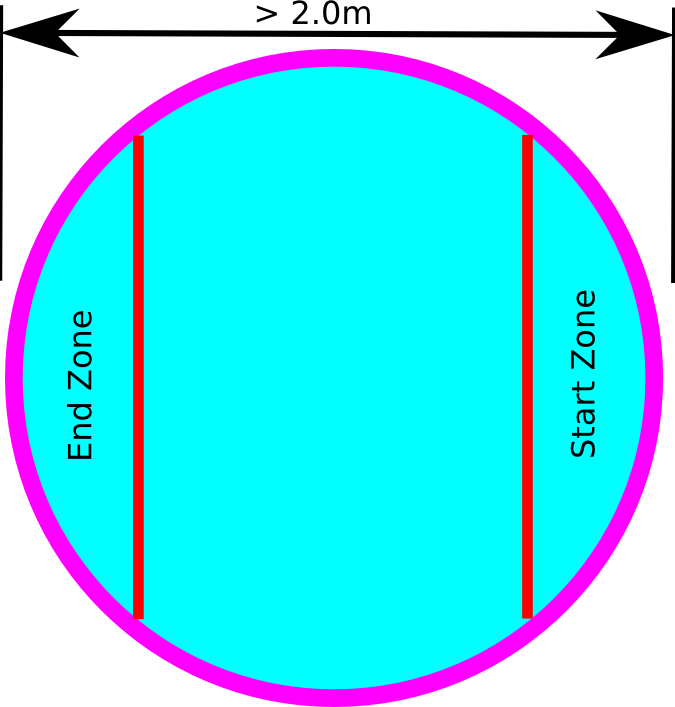
\includegraphics[width=0.4\linewidth]{Figures/dbc-field} \\
\end{tabular}
\caption{Image of a suitable Kiddie Pool and Required Field Markings}
\label{fig:kiddie-pool}
\end{center}
\end{figure}

\item A line indicating the start zone must be indicated at the side
  and bottom of the kiddie pool.

\item A line indicating the end zone must be indicated at the side and
  bottom of the kiddie pool.

\end{lawlist}

\law[DBC]{Items and Tools}
\label{dbc-iteams-and-tools}

\begin{lawlist}[DBC]

\item \label{dbc-items} The minimum set of items that needs to be
  provided for each team are:

  \begin{itemize}
    \item 10 popsicle sticks,
    \item 4 chop sticks,
    \item 2 sheets of paper 
    \item 1 sheet of plastic,
    \item 2 paper cups,
    \item 10 rubber bands,
    \item 10 paper clips,
    \item 1 roll of scotch tape,
    \item 1 wood glue,      
  \end{itemize}
  Other items should be added if possible.

\item \label{dbc-tools} The minimum set of items that needs to be
  provided for each team are:

  \begin{itemize}
    \item 1 wire cutter to cut the chopsticks and popsicle sticks
    \item 3 pens,
  \end{itemize}
  Other tools should be added if possible.

\item \label{dbc-additional} The organizers also must provide a set of
  simulated zongzi for each teams. The simulated zongzi should be
  small, green in colour and roughly pyramid shaped.

\end{lawlist}

\law[DBC]{Game Play}
\label{dbc-game-play}

\begin{lawlist}[DBC]

\item The challenge task for this event is to build a boat that can
  carry a simulated zongzi from the start zone and drop a zongzi into
  the water inside of the end zone.

\item The zongzi is considered to be dropped in the end zone
  successfully only if at least part of both, the zongzi and the boat
  are in the end zone at the time of the drop.

\item Each team has a maximum of three trials for this challenge. The
  best performance according to the scoring formula \ref{dbc-winner}
  will be used.

\item The maximum time for a single trial for a team is 1 minute.

\end{lawlist}

\law[DBC]{Method of Scoring}

\begin{lawlist}[DBC]

\item \label{dbc-winner} The winner of this challenge will be
  determined as follows:
  \begin{enumerate}
    \item teams that are able to complete the full challenge (that is,
      carry a zongzi from the start zone to the end zone and then drop
      it into the water are ranked first. The teams within this group
      are ranked by the time it took from start until the zongzi was
      dropped into the water.
    \item teams that are able to reach the end zone, but unable to
      drop the zongzi successfully will be ranked next. The teams
      within this group are ranked by the time it took from start
      until the boat reached the end zone.
    \item all other teams are awarded 0 points
  \end{enumerate}

\end{lawlist}

\end{document}


% *** Local Variables: ***
% *** mode: LaTeX ***
% *** mode: outline-minor ***
% *** mode: auto-fill ***
% *** outline-regexp: "% !\\|\\\\\\(sub\\)*section" ***
% *** TeX-command-default: "LaTeX PDF" ***
% *** End: ***
